\documentclass[11pt]{article}




%------------------------------------------------------------------
% PROBLEM, PART, AND POINT COUNTING...

% Create the problem number counter.  Initialize to zero.
\newcounter{problemnum}

% Specify that problems should be labeled with arabic numerals.
\renewcommand{\theproblemnum}{\arabic{problemnum}}


% Create the part-within-a-problem counter, "within" the problem counter.
% This counter resets to zero automatically every time the PROBLEMNUM counter
% is incremented.
\newcounter{partnum}[problemnum]

% Specify that parts should be labeled with lowercase letters.
\renewcommand{\thepartnum}{\arabic{problemnum}.\arabic{partnum}}

% Make a counter to keep track of total points assigned to problems...
\newcounter{totalpoints}

% Make counters to keep track of points for parts...
\newcounter{curprobpts}		% Points assigned for the problem as a whole.
\newcounter{totalparts}		% Total points assigned to the various parts.

% Make a counter to keep track of the number of points on each page...
\newcounter{pagepoints}
% This counter is reset each time a page is printed.

% This "program" keeps track of how many points appear on each page, so that
% the total can be printed on the page itself.  Points are added to the total
% for a page when the PART (not the problem) they are assigned to is specified.
% When a problem without parts appears, the PAGEPOINTS are incremented directly
% from the problem as a whole (CURPROBPTS).


%---------------------------------------------------------------------------


% The \problem environment first checks the information about the previous
% problem.  If no parts appeared (or if they were all assigned zero points,
% then it increments TOTALPOINTS directly from CURPROBPTS, the points assigned
% to the last problem as a whole.  If the last problem did contain parts, it
% checks to make sure that their point values total up to the correct sum.
% It then puts the problem number on the page, along with the points assigned
% to it.

\newenvironment{problem}[1]{
% STATEMENTS TO BE EXECUTED WHEN A NEW PROBLEM IS BEGUN:
%
% Increment the problem number counter, and set the current \ref value to that
% number.
\refstepcounter{problemnum}
%
% Add some vspace to separate from the last problem.
\vspace{0.15in} \par
%
\setcounter{curprobpts}{#1} \setcounter{totalparts}{0}	% Reset counters.
%
% Now put in the "announcement" on the page.
{\Large \bf \theproblemnum. \normalsize ({\it \arabic{curprobpts} point\null\ifnum \value{curprobpts} = 1\else s\fi}\/)}
}{
% STATEMENTS TO BE EXECUTED WHEN AN OLD PROBLEM IS ENDED:
%
% If no parts to problem, then increment TOTALPOINTS and PAGEPOINTS for the
% entire problem at once.
\ifnum \value{totalparts} = 0
	\addtocounter{totalpoints}{\value{curprobpts}}	% Add pts to total.
	\addtocounter{pagepoints}{\value{curprobpts}}	% Add pts to page total.
%
% If there were parts for the problem, then check to make sure they total up
% to the same number of points that the problem is worth. Issue a warning
% if not.
\else \ifnum \value{totalparts} = \value{curprobpts}
	\else \typeout{}
	\typeout{!!!!!!!   POINT ACCOUNTING ERROR   !!!!!!!!}
	\typeout{PROBLEM [\theproblemnum] WAS ALLOCATED \arabic{curprobpts} POINTS,}
	\typeout{BUT CONTAINS PARTS TOTALLING \arabic{totalparts} POINTS!}
	\typeout{}
	\fi
\fi
}


%---------------------------------------------------------------------------


% The \newpart command increments the part counter and displays an appropriate
% lowercase letter to mark the part.  It adds points to the point counter
% immediately.  If 0 points are specified, no point announcement is made.
% Otherwise, the announcement is in scriptsize italics.

\newcommand{\newpart}[1]
{
\refstepcounter{partnum}	% Set the current \ref value to the part number.
%\hspace{0.0in}		% Indent the part by a quarter inch.
%
% If points are to be printed for this problem (signaled by point value > 0),
% then put them in in scriptsize italics.
\ifnum #1 > 0
	\makebox[0.5in][l]{{\bf \thepartnum.} {\bf ({\it #1 pt\ifnum #1 = 1\else s\fi\/}) \,\,}}
\else
	\makebox[0.25in][l]{({\bf \thepartnum})}
\fi
%
\hspace{0.1in}		% Lead the material away from the part "number".
%
\addtocounter{totalparts}{#1}	% Add points to totalparts for this problem.
\addtocounter{pagepoints}{#1}	% Add points to total for this page.
\addtocounter{totalpoints}{#1}	% Add points to total for entire test.
}


%---------------------------------------------------------------------------



% Just in case you want to skip some numbers in your test...

\newcommand{\skipproblem}[1]{\addtocounter{problemnum}{#1}}



%---------------------------------------------------------------------------


% The \showpoints command simply gives a count of the total points read in up to
% the location at which the command is placed.  Typically, one places one
% \showpoints command at the end of the latex file, just prior to the
% \end{document} command.  It can appear elsewhere, however.

\newcommand{\showpoints}
{
\typeout{}
\typeout{====> A TOTAL OF \arabic{totalpoints} POINTS WERE READ.}
\typeout{}
}


%---------------------------------------------------------------------------


\setlength\parindent{0pt}

\usepackage{fullpage}
\usepackage{graphicx}
\usepackage[english]{babel}
\usepackage[latin1]{inputenc}
\usepackage{times}
\usepackage[T1]{fontenc}
\usepackage{amsmath}
\usepackage{amssymb}
\usepackage{enumerate}

\newcommand{\argmax}{\mathop{\arg\max}}
\newcommand{\deriv}[1]{\frac{\partial}{\partial {#1}} }
\newcommand{\dsep}{\mbox{dsep}}
\newcommand{\Pa}{\mathop{Pa}}
\newcommand{\ND}{\mbox{ND}}
\newcommand{\De}{\mbox{De}}
\newcommand{\Ch}{\mbox{Ch}}
\newcommand{\graphG}{{\mathcal{G}}}
\newcommand{\graphH}{{\mathcal{H}}}
\newcommand{\setA}{\mathcal{A}}
\newcommand{\setB}{\mathcal{B}}
\newcommand{\setS}{\mathcal{S}}
\newcommand{\setV}{\mathcal{V}}
\DeclareMathOperator*{\union}{\bigcup}
\DeclareMathOperator*{\intersection}{\bigcap}
\DeclareMathOperator*{\Val}{Val}
\newcommand{\mbf}[1]{{\mathbf{#1}}}
\newcommand{\eq}{\!=\!}
\newcommand{\cut}[1]{}

\begin{document}

{\centering
  \rule{6.3in}{2pt}
  \vspace{1em}
  {\Large
    CS688: Graphical Models - Spring 2018\\
    Assignment 3\\
  }
  \vspace{1em}
  Assigned: Tuesday, March 13th. Due: Tuesday, March 27th 11:59pm\\
  \vspace{0.1em}
  \rule{6.3in}{1.5pt}
}\vspace{1em}

\textbf{Getting Started:} You should complete the assignment using your own installation of Python 2.7. The only modules you are permitted to use in your implementations are Numpy, SciPy, and Scikit-Learn. To get started with the code portions of the assignment, download the assignment archive from Moodle and unzip the file. The data files for this assignment are in the \texttt{data} directory. Code templates are in the \texttt{code} directory.\\

\textbf{Deliverables:} This assignment has two types of deliverables: a report and code files.

\begin{itemize}
\item \textbf{Report: } The solution report will give your answers to the homework questions. Items that you should include in your report are marked with \textbf{(report)}. The maximum length of the report is 5 pages in 11 point font, including all figures and tables. You can use any software to create your report, but your report must be submitted in PDF format. You will upload the PDF of your report to Gradescope under \verb|HW03-Report| for grading. It is strongly recommended that you typeset your report. To assist with this if you wish to use Latex, the Latex source of the handout is also included in the homework archive.

\item \textbf{Code: } The second deliverable is your code. Items that you should include in your code are marked with \textbf{(code)}.  Your code must be Python 2.7 (no iPython notebooks, other formats, or code from other versions of Python). You will upload a zip file (not rar, bz2 or other compressed format) containing all of your code to Gradescope under \verb|HW03-Programming|.  When unzipped, your zip file should produce a directory called \verb|code|. Do not 
upload the data directory to Gradescope.

\end{itemize}
\vspace{0.5em}

\textbf{Academic Honesty Statement:} Copying solutions from external
sources (books, web pages, etc.) or other students is considered
cheating. Sharing your solutions with other students is also
considered cheating. Collaboration indistinguishable from copying is a violation 
of the course's collaboration policy and will be treated as cheating.
Any detected cheating will result in a grade of 0
on the assignment for all students involved, and potentially a grade
of F in the course.\\


\textbf{Introduction:} In this assignment, you will experiment with two sampling-based methods for inference. The first question focuses on the use of Monte Carlo methods for human activity recognition with missing data. In this problem, a total of four on-body sensors are used to collect data. There is one heart rate sensor and three inertial measurement devices that each include several sensors (3-axis accelerometer, 3-axis gyroscope, 3-axis magnetometer). The problem is that wireless connectivity can be lost between different sensing devices and the data recording device, resulting in missing data. You will develop a method for making predictions in the presence of missing observations.\\

The second question focuses on approximating queries for Bayesian networks using Gibbs sampling. The key strength of Bayesian network models is that they can be used to answer arbitrary queries once they have been learned. However, the complexity of inference can be high for queries requiring extensive marginalization. In this question, you will develop a Gibbs sampler that can be used to answer arbitrary probability queries for the Heart Disease Bayesian network given a learned set of model parameters.
\\

\begin{problem}{50} \textbf{Human Activity Recognition with Missing Data:} Typical probabilistic discriminative learning methods
aim  to learn a model of the form $P(Y=y|\mbf{X}=\mbf{x})$ where $y$ is a class label and $\mbf{x}$ is a feature vector. However,
such models can not be applied when the feature vector $\mbf{x}$ contains missing observations. To deal with such cases,
we can also learn a model $P(\mbf{X}=\mbf{x})$ over the feature space. The joint model becomes:

$$P(Y=y,\mbf{X}=\mbf{x})=P(Y=y|\mbf{X}=\mbf{x})P(\mbf{X}=\mbf{x})$$

We let $\mbf{x}^m$ indicate the missing values of $\mbf{x}$, and $\mbf{x}^o$ indicate the observed values. The classification
problem given missing data becomes:

$$P(Y=y|\mbf{X}^o=\mbf{x}^o)=\int P(Y=y|\mbf{X}^o=\mbf{x}^o,\mbf{X}^m=\mbf{x}^m)P(\mbf{X}^m=\mbf{x}^m|\mbf{X}^o=\mbf{x}^o)d\mbf{x}^m$$

In this question, you will use a multi-class (softmax) logistic regression model $P(Y=y|\mbf{X}=\mbf{x},\theta)\propto \exp(\mbf{w}_y\mbf{x}+b_y)$,
and a multivariate Gaussian model $P(\mbf{X}=\mbf{x}|\mu,\Sigma)=\mathcal{N}(\mbf{x};\mu,\Sigma)$. Note that $\theta$ refers to the set of all
logistic regression model parameters.\\

\newpart{5} Derive the formula for $P(Y=y|\mbf{X}^o=\mbf{x}^o)$ shown above starting from the definition of the joint
distribution $P(Y=y,\mbf{X}=\mbf{x})$. (report)\\

\newpart{5} Provide an analytic expression for $P(\mbf{X}^m=\mbf{x}^m|\mbf{X}^o=\mbf{x}^o)$ given that 
$P(\mbf{X}=\mbf{x})=\mathcal{N}(\mbf{x};\mu,\Sigma)$. (Hint you will want to refer to the multivariate Gaussian
conditioning rules). (report)\\

\newpart{5} Even given the model parameters $\theta$, $\mu$, $\Sigma$, computing $P(Y=y|\mbf{X}^o=\mbf{x}^o)$
is still difficult because the required integral is not analytically tractable.
Describe how $P(Y=y|\mbf{X}^o=\mbf{x}^o)$ can instead be approximated by a Monte Carlo average. Then, describe 
how actual predictions can be made. (report)\\

\newpart{10} Complete the implementation of the code in \verb|mclrmiss.py|. In particular,
the \verb|fit| function should learn the parameters $\theta$ of the softmax logistic regression classifier
(you will use scikit-learn's implementation) and the parameters $\mu$ and $\Sigma$ of the multivariate 
Gaussian (you should implement this from scratch in Numpy). Note that completely observed data are 
available for training these models. In the \verb|predict| and \verb|predict_proba| functions, you will 
implement the prediction methods that you described as the answer to the previous question. (code)\\

\newpart{10} In this question, you will apply your classifier to the test set. The test set contains
a mixture of complete data cases, and data cases missing different numbers of feature values. Missing values 
are indicated via Nan's. Report the classification error rate you find on the test set, as well as
the average conditional log likelihood of the test data. Use 10 samples per data case. Report the same 
values obtained by using a simple zero imputation strategy where all missing values are filled in 
with zeros.  Add your code for this experiment to \verb|experimentsQ1.py|. (report)\\

\newpart{15} Finally, you will analyze the impact of missing data on classification. Describe an
experiment that uses the trained classifier and the test data set to assess how the amount of 
missing data impacts the classification error rate and the average conditional log likelihood 
of the test cases. Conduct your experiment and report the results using a pair of figures,
one for the  error rate and one for the average conditional log likelihood. The x-axes
should correspond to the amount of missing  data.  Repeat your analysis using simple zero imputation and provide 
corresponding figures. Comment on how missing data affects the test error compared to the 
test log likelihood, and how modeling $P(X)$ compares to simply imputing zeros for all missing values. 
Add your code for this experiment to \verb|experimentsQ1.py|. (report)\\

\end{problem}
	

\begin{problem}{50} \textbf{Heart Disease Network Queries:} In this question, we will re-visit 
the problem of computing queries for the heart disease network from Homework 1 using Gibbs sampling.
We will follow the general inference strategy of converting the Bayesian network into a Markov network,
and performing inference in the Markov Network. As a reminder, the network structure is given
below.
\begin{center}
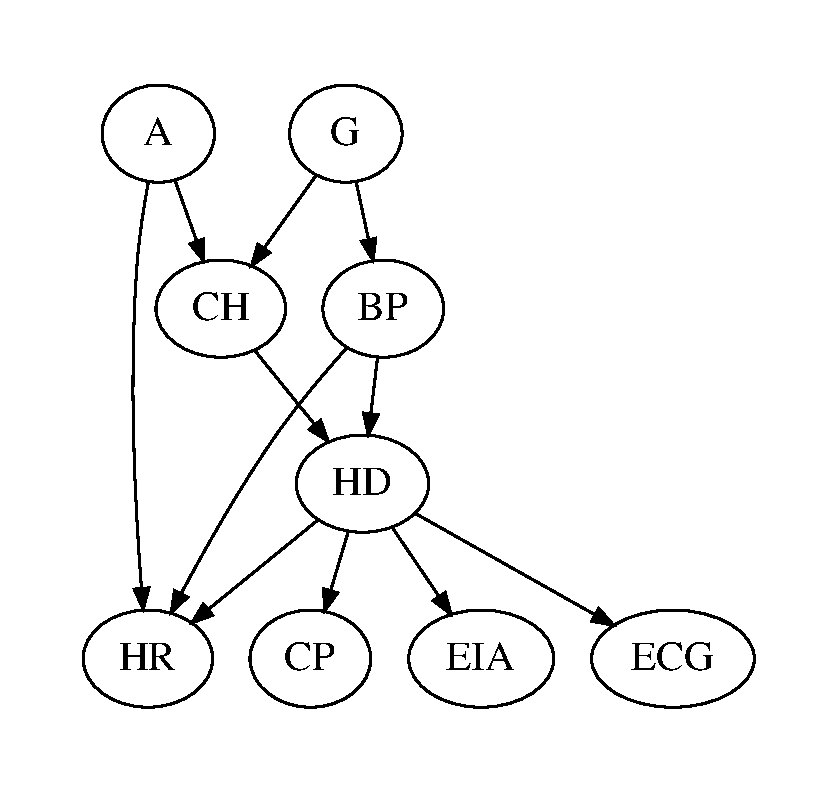
\includegraphics[width=3in]{figures/bn.pdf}
\end{center}

\newpart{5} Find a Markov network that is a minimal I-map for the heart disease network.
Provide a figure showing your Markov network. (report)\\

\newpart{5} Provide a list of the factors in the Markov network (with their scopes), indicating 
which CPT each factor corresponds to. (report)\\

\newpart{5} Provide a table with one row per variable listing the variable and the Markov blanket for 
that variable in the MRF. List the rows in alphabetical order by variable name. (report)\\

\newpart{10} For each variable in the Markov network, provide an expression for the conditional probability of that
variable given all of the other variables in the network in terms of the factors in your network. 
Simplify where possible using the Markov blanket of each variable.  (report)\\

\newpart{10} Suppose we partition the variables in the network into three sets $\mbf{X}$, $\mbf{Y}$, and $\mbf{Z}$.
Explain how to use the Gibbs sampler to approximate $P(\mbf{X}|\mbf{Z})$. Provide pseudo-code for an
algorithm implementing this computation. (report)\\

\newpart{10} Complete the implementation of the code in \verb|mrf.py|.
A set of learned Bayesian network parameters for the Heart Disease model
are provided to initialize the MRF model parameters. You will complete
the \verb|__init__| method to initialize the MRF model parameters from the 
Bayesian networks parameters. You may hard-code the structure of the MRF.
You will also complete the function 
\verb|conditional|, which computes the conditional distribution over a single
variable given values for all other variables, and the function 
\verb|gibbs_query|, which uses Gibbs sampling to approximately answer an
arbitrary probability query. The results of querying are returned 
using instances of the \verb|prob_table| class. You will also need to
implement this class, which has a single required member function. 
The API's for both classes are documented within the provided code templates.
You  may create any additional functions or classes that you like, but do not
modify the function signatures unless this is specifically indicated as
being allowed in the docstring for a function. Make sure to 
submit  any additional code files that you create. (code)\\

\newpart{5} Use your implementation to provide answers for each of the following 
queries. Provide your answers as a set of tables. Use 10,000 samples for each query. 
Add your code for this experiment to \verb|experimentsQ2.py|.\\

\begin{enumerate}[(a)]
	\item $P(A|CP=``Atypical")$
	\item $P(HD|CH=``H",HR=``L")$
	\item $P(ECG|HD=``N", HR=``L")$
	\item $P(CH,BP|EIA="N")$
	\item $P(G, HD|CP=``Typical",HR=``H")$	
\end{enumerate}	


\end{problem}


\showpoints
\end{document} 